\documentclass{standalone}
\usepackage{pgfplots}
\pgfplotsset{compat=newest}

\begin{document}

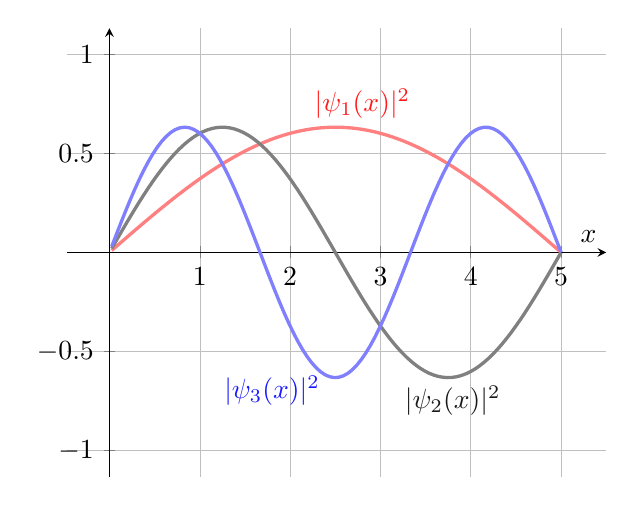
\begin{tikzpicture}

\begin{axis}
    [grid=both,
     samples=200,
     xlabel=$x$,
     ylabel=$$,
     grid style={line width=.1pt, draw=gray!10},
     major grid style={line width=.2pt,draw=gray!50},
     axis lines=middle,
     restrict y to domain=-1.:5.,
     restrict x to domain=0:5,
     enlargelimits={abs=0.5}
    ]

    \addplot [very thick, red!50] {sqrt(2/5)*sin((deg(1*x*pi/5)))};
    \node[red!90] at (2.8, .75) {$|\psi_1(x)|^2$};
    \addplot [very thick, black!50] {sqrt(2/5)*sin((deg(2*x*pi/5)))};
    \node[black!90] at (3.8, -0.75) {$|\psi_2(x)|^2$};
    \addplot [very thick, blue!50] {sqrt(2/5)*sin((deg(3*x*pi/5)))};
    \node[blue!90] at (1.8, -0.7) {$|\psi_3(x)|^2$};
  
\end{axis}
\end{tikzpicture}
\end{document}
